\chapter{绪论}\label{chap:introduction}

\section{研究背景与意义}

在全球科技迅猛发展的浪潮中，机器人技术（Robotics）已崛起为驱动社会进步与产业变革的核心驱动力。习近平总书记深刻指出，要“以科技创新推动产业创新，积极培育新能源、新材料、先进制造、电子信息等战略性新兴产业，积极培育未来产业，加快形成新质生产力，增强发展新动能”。作为衡量国家科技创新与高端制造水平的关键标志，机器人技术不仅是军事与商业领域的前沿焦点，更是全球竞逐的战略新高地。对此，我国政府高度重视，连续出台多项政策，旨在系统推进机器人技术的自主创新与深度应用。《“十四五”机器人产业发展规划》\cite{miit2021} 强调了机器人技术在制造业、服务行业和特种领域的应用，并提出了到 2025 年实现制造业机器人密度较 2020 年翻番的目标。工信部 2023 年发布的《“机器人+”应用行动实施方案》\cite{miit2023} 进一步提出，到 2025 年制造业机器人密度较 2020 年实现翻番。

地面移动机器人作为现有机器人中的绝对主流，越来越多地被用于工业生产、生活娱乐、搜救任务、军事侦察等场景中。在地面移动机器人的众多构型中，轮式机器人具有运动速度快、控制简单、能耗低等优点，但在非结构化地形（如楼梯、碎石、斜坡等）中的适应能力较差；而足式机器人虽具备良好的越障能力，但在平坦环境中运行时，在能效和运动速度方面落后于轮式机器人。为兼顾轮式机器人的高效性与足式机器人的地形适应性，轮足复合式机器人成为当前机器人研究的热点之一\cite{ding2024}。当前，主流研究聚焦于四足轮腿式机器人\cite{hutter2016}。该类机器人采用分布式腿部关节与轮组相耦合的设计，兼具动态平衡能力与中等障碍物跨越性能。然而，其多足架构也引发了结构冗余问题。以典型四足轮腿式机器人为例，其通常需配置 16 个以上的独立执行器，这不仅导致机械结构复杂性呈指数增长，还引入了显著的转动惯量与惯性负载，在控制器设计与建模上也带来了困难。而双轮足机器人作为一种典型的轮足融合构型，既能在平坦路面实现快速移动，又能通过腿部结构实现越障、上下楼梯等复杂动作，在结构上更加简单，具有重要的研究价值与应用前景。

在双轮足机器人机械结构上，主流设计分为串联、并联和混合式。串联结构工作空间大，但刚度和承载能力偏弱；并联结构刚度和承载力强，但运动空间受限。因此，本研究选择了混合式结构作为方向，它通过在串联主链中引入局部并联支链，旨在兼顾运动灵活性与结构刚性，从硬件基础上优化机器人的性能。在运动控制上，像 WBC（全身控制）、MPC（模型预测控制）这类高级算法虽然性能强大，但它们严重依赖高精度模型，计算复杂；而强化学习（RL）则需要海量的训练数据。这些都对机器人的实时控制和嵌入式部署提出了挑战。因此，本研究计划避开这条“重”路线，转向一种基于物理直觉的轻量级混合控制方案，以期在保证性能的同时，实现更高效的实时控制。总体来说，本课题旨在完成双轮足机器人的混合式腿部结构设计，同时提出一种结合 LQR（线性二次调节器）与 VMC（虚拟模型控制），并引入轻量级 QP（二次规划）的轻量级混合控制方案。

\section{双轮足机器人机械结构设计国内外研究现状与分析}

\subsection{串联结构}

串联结构因其结构简单、控制灵活，被广泛应用于双轮足机器人中。波士顿动力公司在 2017 年首次展示了具有惊人运动能力的 Handle 轮腿机器人\cite{boston2023handle}，其核心创新在于采用了典型的串联式腿部构型。该构型仿照生物肢体的串联关节设计，由髋关节、膝关节及踝关节依次连接而成，形成了开链的运动结构。这种设计赋予了机器人巨大的灵活性与充裕的工作空间，使其能够通过关节的协调运动，动态调整质心位置，从而在轮式高速移动时维持倒立摆平衡，并在遇到障碍时，通过腿部大幅度的屈伸实现跳跃或越障，完美实现了轮式效率与腿式适应性的融合。随后在 2018 年发布的第二代版本\cite{boston2023stretch}，则进一步在负载与续航方面实现了重要提升，奠定了其在轮腿复合机器人领域的标杆地位。

\begin{figure}[H]
  \centering
  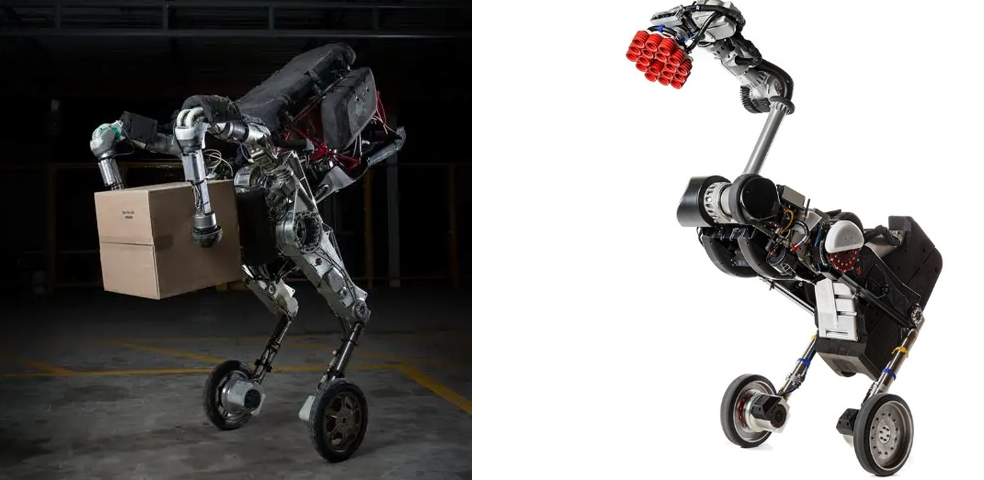
\includegraphics[width=0.55\textwidth]{figures/ch01/image3.png}
  \caption{一代 Handle 机器人（左），二代 Handle 机器人（右）}
\end{figure}

2023 年，浙江大学公开的双轮足机器人 HotWheel\cite{yu2023hotwheel}，在机械构型上采用了先进的串联式腿部设计。其单腿具备三个主动自由度，相较于同期主流双轮足平台（如 Ascento、Ollie 等）通常仅有的两个自由度，HotWheel 在髋关节处关键性地增加了一个侧摆自由度。这一串联构型使其腿部成为一个在空间内具有高度灵活性的开链机构，不仅极大地扩展了足端（轮心）的工作空间，更使机器人能够通过主动的侧向运动来动态调整重心，从而实现了在 V 型斜坡等复杂地形上的稳定驻留与敏捷运动。

\begin{figure}[H]
  \centering
  \begin{minipage}[b]{0.37\textwidth}
    \centering
    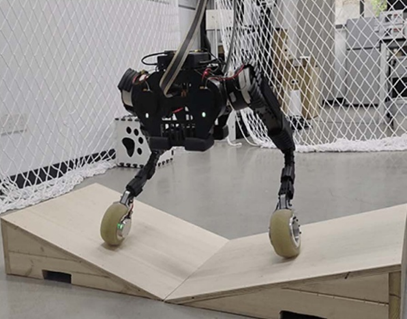
\includegraphics[width=\textwidth]{figures/ch01/image4.png}
  \end{minipage}
  \begin{minipage}[b]{0.37\textwidth}
    \centering
    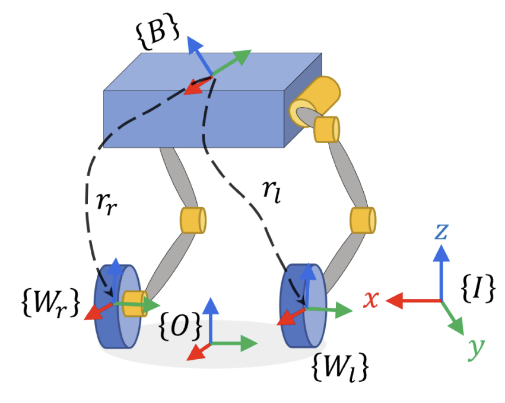
\includegraphics[width=\textwidth]{figures/ch01/image5.png}
  \end{minipage}
  \caption{HotWheel 机器人}
\end{figure}

2024 年，逐际动力推出了 TRON 1 多形态双足机器人\cite{limx2025tron1}，其腿部采用了典型的三自由度串联构型。这种开放链式结构为其带来了广阔的工作空间与高度的运动灵活性，是机器人能够通过更换足端，灵活切换点足、双足及双轮足等多种形态，以适应不同场景需求的结构基础。

\begin{figure}[H]
  \centering
  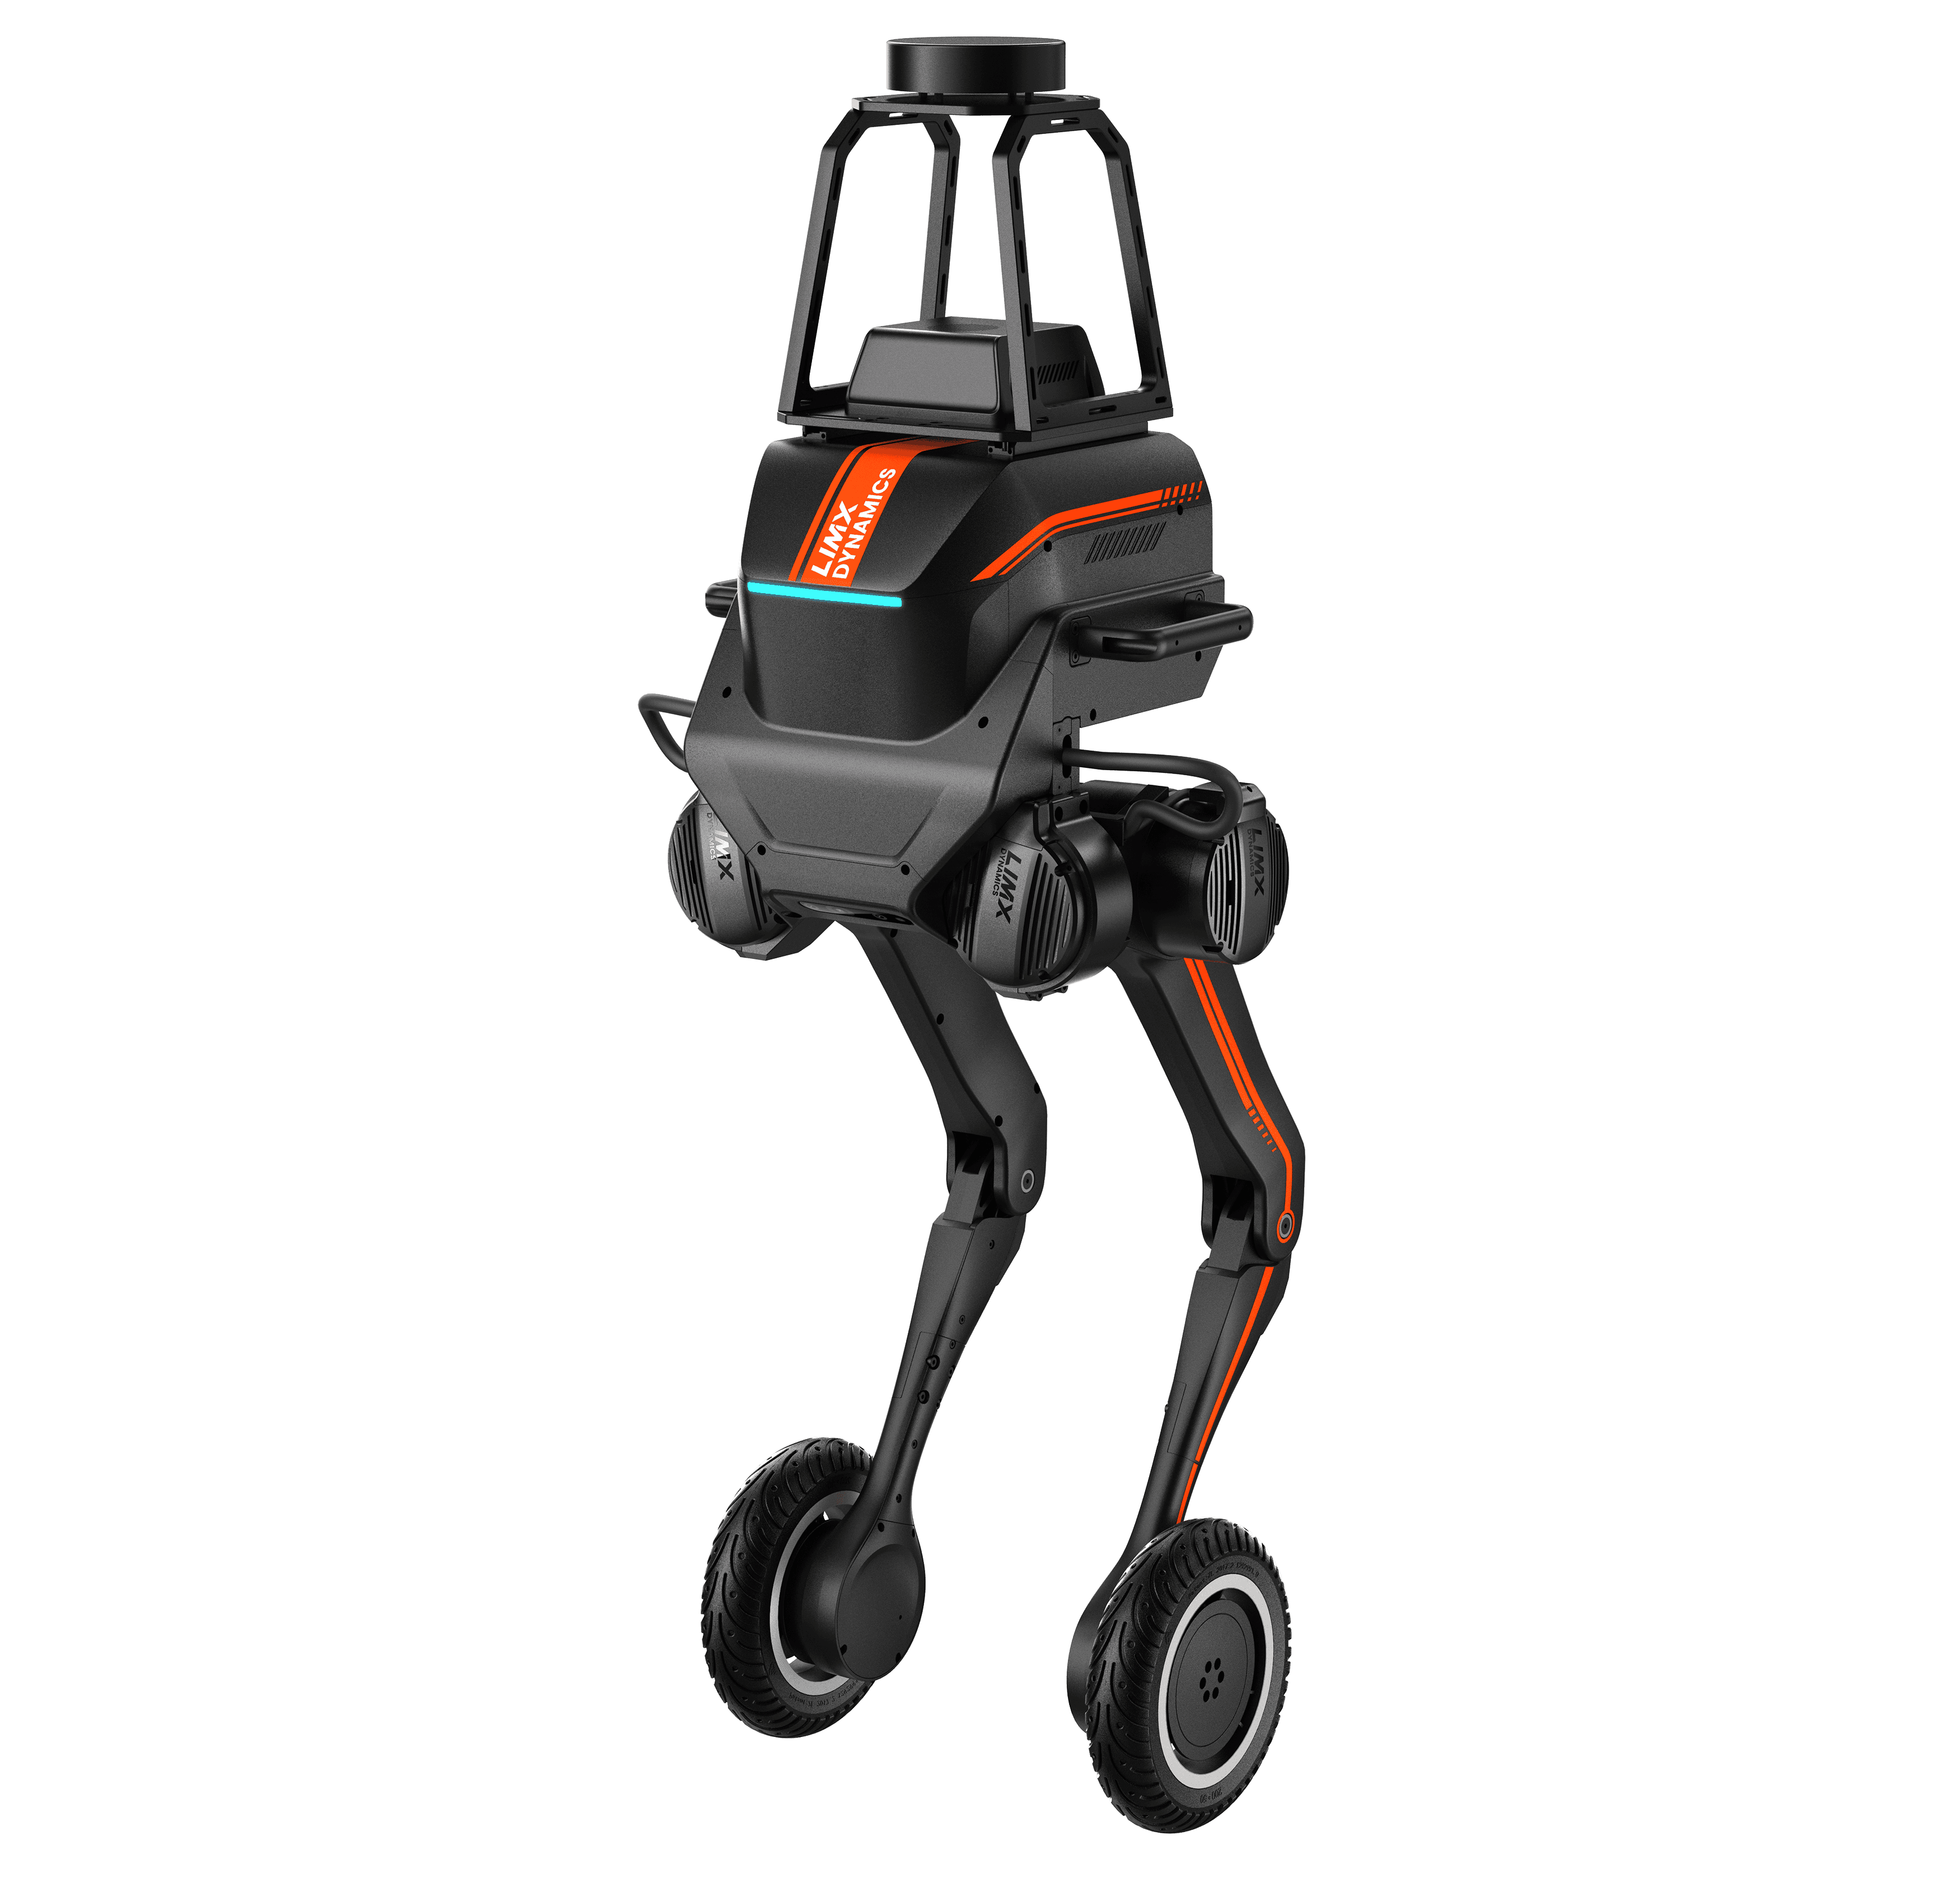
\includegraphics[width=0.45\textwidth]{figures/ch01/image6.png}
  \caption{TRON 1 机器人}
\end{figure}

\subsection{并联结构}

并联结构因其结构稳定、承载能力强，逐渐成为双轮足机器人设计的重要方向。

2004 年，日本 Sugahara 与 Hashimoto 团队在轮足复合机器人领域进行了系列研究。他们首先研制了双足载人机器人 WL-16\cite{sugahara2004}，随后又开发了新型轮式脚踏系统 WS-2\cite{hashimoto2005}。通过将 WS-2 与 WL-16 组合，他们构建了一种新颖的轮足复合机器人系统。该系统的腿部采用 6 自由度并联机构，能实现精准的足底姿态控制。其核心功能在于可依据地形需求，动态切换运动模式：放下足底橡胶垫时可执行稳定的足式步态；收起橡胶垫使轮胎触地后，则可进行高效的轮式移动。

\begin{figure}[H]
  \centering
  \begin{minipage}[b]{0.22\textwidth}
    \centering
    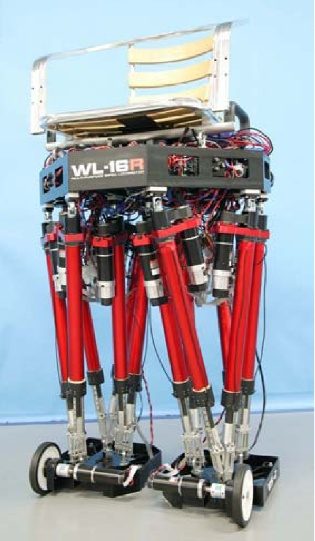
\includegraphics[width=\textwidth]{figures/ch01/image7.jpeg}
  \end{minipage}
  \begin{minipage}[b]{0.45\textwidth}
    \centering
    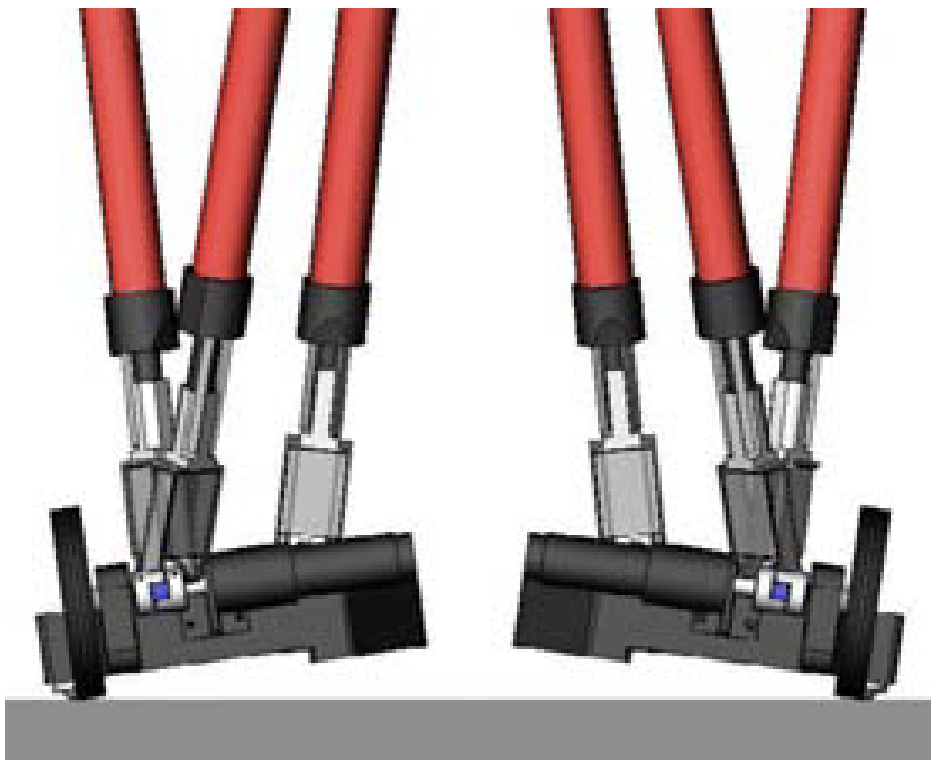
\includegraphics[width=\textwidth]{figures/ch01/image8.png}
  \end{minipage}
  \caption{WS-2 / WL-16}
\end{figure}

2019 年，苏黎世联邦理工学院（ETH Zurich）推出的 Ascento 轮腿式机器人\cite{klemm2019ascento}，采用闭式四连杆结构。该机构经过优化，能使足端（轮心）在垂直方向上近似线性运动。这种独特设计有效解耦了机器人的跳跃与平衡控制，使得其在起跳和落地时躯干姿态保持稳定。腿部结构件均基于拓扑优化方法设计并借助 3D 打印技术制造，在保证结构强度的同时实现了轻量化。此外，髋关节内置的卷簧有效平衡了机身自重，既降低了保持站立时的控制能耗，也提升了其跳跃性能。

\begin{figure}[H]
  \centering
  \begin{minipage}[b]{0.35\textwidth}
    \centering
    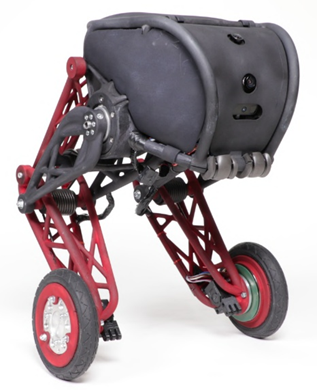
\includegraphics[width=\textwidth]{figures/ch01/image9.png}
  \end{minipage}
  \begin{minipage}[b]{0.5\textwidth}
    \centering
    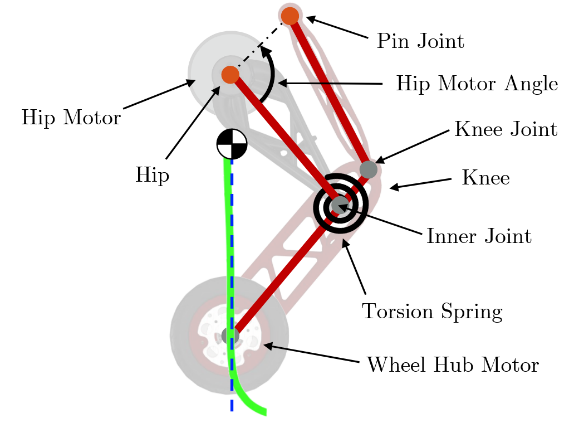
\includegraphics[width=\textwidth]{figures/ch01/image10.png}
  \end{minipage}
  \caption{Ascento 机器人}
\end{figure}

2021 年，腾讯公司发布了双轮足机器人 Ollie\cite{wang2021ollie}。该机器人在机械构型上采用对称五连杆设计，其单腿集成了一个轮毂电机与两个关节电机。此构型不仅简化了控制系统，还使其驱动轮轮心能够易于实现精确的直线运动轨迹。为增强其在空中的姿态调整能力，Ollie 在机身腹部创新性地增加了一个主动飞轮（出力杆）。该飞轮通过高速转动产生的角动量，可有效补偿机体在跳跃时因欠驱动特性产生的姿态偏差。凭借其高度紧凑的设计，Ollie 的最低身高仅 0.35 米，但却能完成跳上 0.4 米台阶、实现 0.6 米的竖直起跳高度，甚至完成 360 度空翻等高动态动作，展示了其出色的运动能力与控制水平。

\begin{figure}[H]
  \centering
  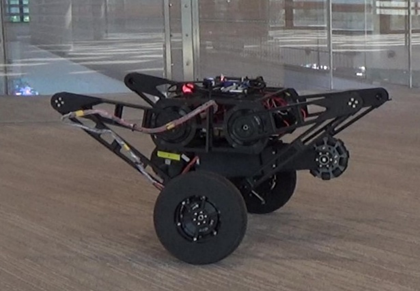
\includegraphics[width=0.52\textwidth]{figures/ch01/image11.png}
  \caption{Ollie 机器人}
\end{figure}

\subsection{混合式结构}

2021 年，开源项目 Stanley 机器人\cite{stanley2025} 的腿部采用了一种巧妙的串并联混合构型，这使其在同类开源足式机器人中独具特色。具体而言，其单条腿在宏观上呈现为一个典型的三自由度串联链，由髋关节横滚、髋关节俯仰和膝关节俯仰依次连接而成，这保证了机器人腿部拥有足够大的灵活工作空间。然而，其核心创新在于驱动方式的并联化。髋关节俯仰和膝关节俯仰的驱动电机并联地集中布置在机身内部，并通过独立的绞盘和线缆将动力远程传递至各个关节。这种设计融合了两种构型的优势：它既继承了串联腿运动灵活、工作空间大的优点，又通过驱动并联化，将沉重的电机移至机体，显著降低了腿部的运动惯量，并利用绞盘机构实现了高扭矩输出与低反向间隙。

\begin{figure}[H]
  \centering
  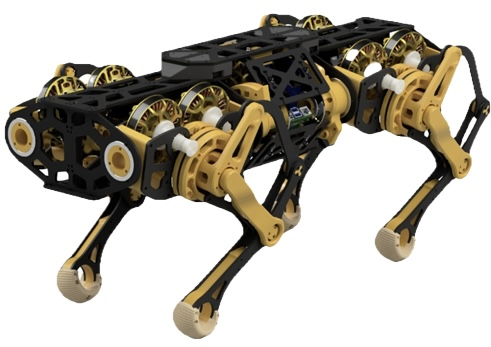
\includegraphics[width=0.38\textwidth]{figures/ch01/image12.jpg}
  \caption{Stanley 机器人}
\end{figure}

2025 年，上海交通大学交龙战队开源了一款双轮足机器人\cite{sjtu2025rm}，在腿部结构上实现了关键创新：采用了一种“宏观串联、驱动并联”的混合构型，既能够在运动学上保持串联腿的大工作空间，同时通过相似连杆机构实现并联传动，优化了负载分配与腿部惯量。它还使用了导电滑环使得腿部具有 360° 全向旋转能力，能够在各种姿态下实现倒地自起。该设计结合嵌套式碗组轴承的髋关节轴系与极简的螺丝螺母膝关节，在实现全向摔倒自恢复与碰撞-收腿式越障功能的同时，达到了高刚度与轻量化的平衡，显著提升了机器人在复杂环境下的机动性与运动能力。

\begin{figure}[H]
  \centering
  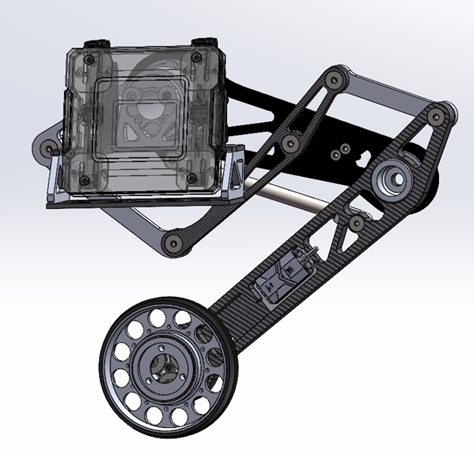
\includegraphics[width=0.4\textwidth]{figures/ch01/image13.png}
  \caption{混合式构型腿部}
\end{figure}

\section{双轮足机器人运动控制策略国内外研究现状与分析}

双轮足机器人的平衡控制和水平运动主要依靠车轮转动实现，而对复杂地形的适应和完成高难度动作则需要腿部结构的配合。双轮足机器人的运动控制策略可视为足式与轮式控制方法的融合，因此当前主流控制方法如线性二次调节器控制（Linear Quadratic Regulator，LQR）、比例积分微分控制（Proportional Integral Derivative control，PID）、模型预测控制（Model Predictive Control，MPC）、滑模控制（Sliding Mode Control，SMC）、虚拟模型控制（Virtual Model Control，VMC）、全身控制（Whole Body Control，WBC）、强化学习控制（Reinforcement Learning Control）均可用于双轮足机器人运动控制。

2001 年，Pratt 等人提出虚拟模型控制（VMC）\cite{pratt2001}，这是一种基于物理直觉的机器人运动控制方法，其核心贡献在于通过模拟虚拟机械元件（如弹簧、阻尼器等）生成关节力矩，从而实现对复杂动态系统（如双足机器人）的直观且高效的控制。该方法不依赖于逆向动力学或精确轨迹跟踪，而是通过构建虚拟力场来“引导”机器人完成期望动作，显著简化了高层任务描述向底层控制的转化过程。论文进一步展示了 VMC 在实物机器人 Spring Turkey 上的成功应用，实现了稳定平地行走，并在仿真中扩展至未知坡度地形行走，体现了该方法在简化控制设计、降低计算需求与增强系统鲁棒性方面的显著优势。

\begin{figure}[H]
  \centering
  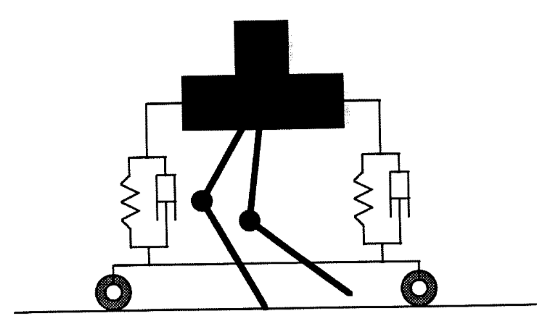
\includegraphics[width=0.55\textwidth]{figures/ch01/image14.png}
  \caption{搭载虚拟助行架的 Spring Turkey 机器人}
\end{figure}

2005 年，Luis Sentis 提出了一种基于分层控制的合成全身行为的统一框架（WBC）\cite{sentis2005}。区别于将约束条件作为次要运动标准来处理的传统方法，作者开创性地将约束，例如关节限制、碰撞和接触，直接集成到控制公式中，并赋予其最高优先级。该框架采用动态一致的零空间投影（Null-Space Projection）技术，将操作任务和姿态控制依次投影到优先级更高任务的零空间中，从而确保在执行复杂操作任务时，高优先级约束永远不会被打破，显著增强了机器人在高不确定性环境中与物理世界进行安全和高效交互的能力。

2020 年，Victor Klemm 提出了 LQR 辅助的全身控制框架\cite{klemm2020lqr}，成功应用于带有运动学闭环（闭式四连杆机构）的轮式双足机器人 Ascento。该方法首先为机器人 Ascento 导出了完整的刚体动力学模型，特别是通过闭环力（Loop Closure Forces）的解析解，以一种可推广的方式处理了腿部的运动学闭环。最关键的是，为了解决轮式平衡机器人固有的非最小相位（non-minimum phase）平衡动力学问题，作者将一个线性二次调节器（LQR）反馈律作为一个运动任务集成到分层 WBC 方案中，从而使控制器能够生成正确的“先向后、再向前”的加速行为以保持平衡。此外，该方案还通过根据零力矩点（ZMP）的位置来调节机器人车体侧倾角，提高了机器人在转弯时抵抗侧翻的鲁棒性。

\begin{figure}[H]
  \centering
  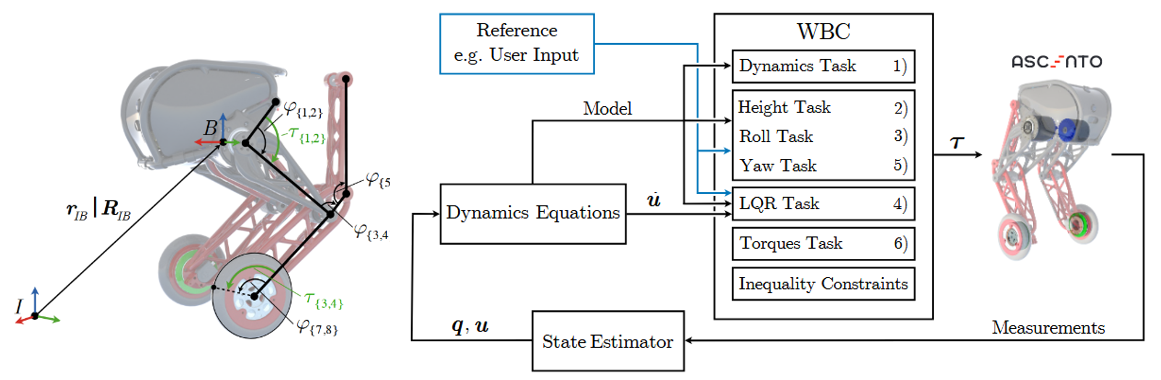
\includegraphics[width=0.82\textwidth]{figures/ch01/image15.png}
  \caption{腿部连杆运动闭环（左），LQR-WBC 控制框架（右）}
\end{figure}

2022 年，Jiajun Wang 提出了 MFT 增强型全身控制方案（MFT-WBC）\cite{wang2022mft}。该方案解决了 MFT 指标与机器人构型之间的非线性关系，通过离线预处理建立机器人的 MFT 优选空间，并将其近似为多面体；随后，该多面体被转化为加速度层面的软不等式约束（通过引入松弛变量）集成到在线的二次规划（QP）优化问题中。这种离线建模与在线 QP 优化相结合的策略，不仅大幅减轻了在线计算负担，实现了 1\,kHz 的高频伺服速率，更重要的是，它确保了机器人在动态任务执行过程中能维持在高传递性配置内，从而显著提升了并联腿式机器人的高速度、高加速度能力，并有效增强了系统对外部冲击和不平坦地形的反应鲁棒性。

\begin{figure}[H]
  \centering
  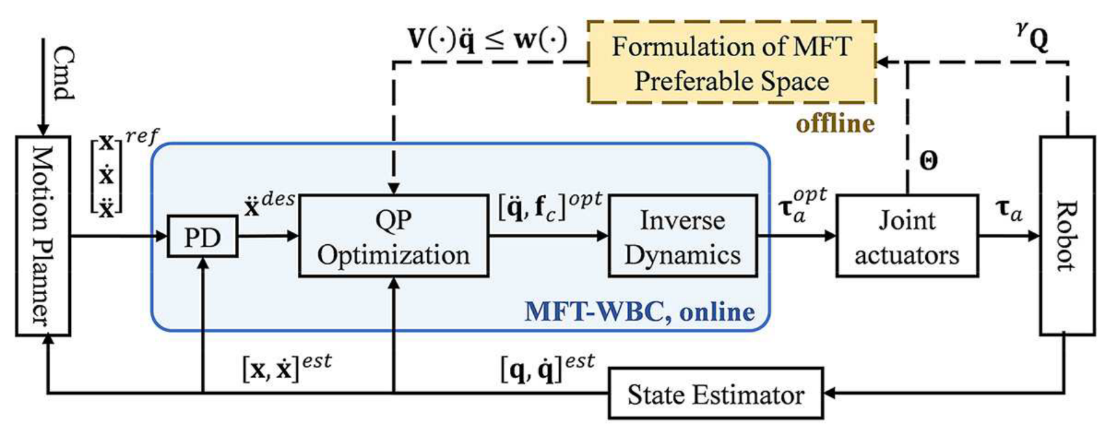
\includegraphics[width=0.72\textwidth]{figures/ch01/image16.png}
  \caption{MFT-WBC 控制框架}
\end{figure}

2022 年，Zhang J 等人创新性地应用了自适应动态规划（ADP）\cite{zhang2022ollie}，通过价值迭代（VI）从机器人的不稳定数据中离线学习初始稳定控制器，并利用策略迭代（PI）在线更新控制策略以快速适应高度、负载等动态变化；同时，将 ADP 生成的平衡参考指令嵌入 WBC 的优化框架，实现了在多任务场景下对机器人全身关节的协调控制。物理实验验证了该框架的强适应性、高鲁棒性以及优异的运动灵活性，显著提升了 Ollie 机器人在复杂地形（如斜坡、台阶）下的自主运动能力。

\begin{figure}[H]
  \centering
  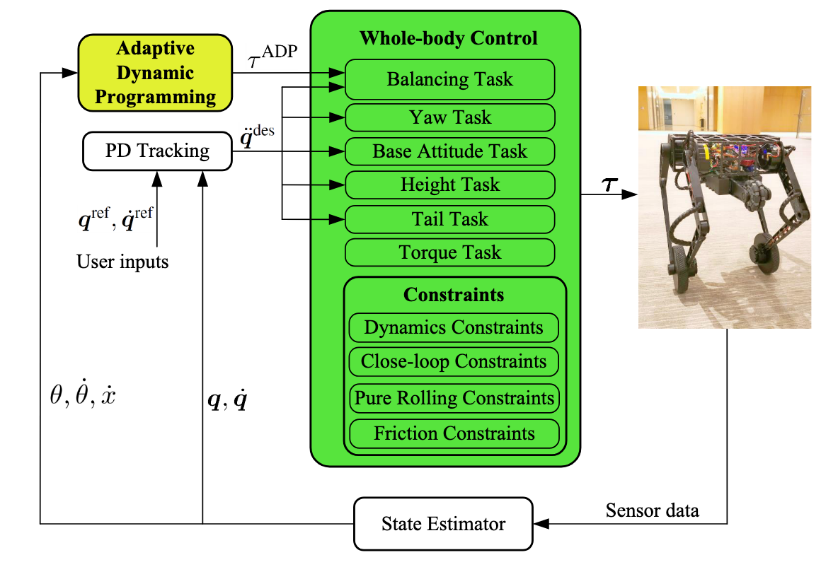
\includegraphics[width=0.8\textwidth]{figures/ch01/image17.png}
  \caption{Ollie 的控制框架}
\end{figure}

2023 年，Jianqiao Yu 提出了一套基于模型预测控制（MPC）的全身姿态跟踪框架\cite{yu2023hotwheel}。研究团队创新性地提出了轮式刚体动力学（WRBD）模型，该模型将机器人躯干视为浮动基，并直接将车轮的非完整约束纳入动力学方程，从而在保证模型精度的同时显著降低了计算复杂度。基于此模型设计的 MPC 控制器，能够实时优化并跟踪躯干的 6 自由度位姿，同时综合考虑动力学约束与执行器极限，最终在实物平台上实现了超越传统 LQR 控制器的轨迹跟踪性能，为轮足机器人在复杂环境下的高动态运动提供了关键技术支撑。

\begin{figure}[H]
  \centering
  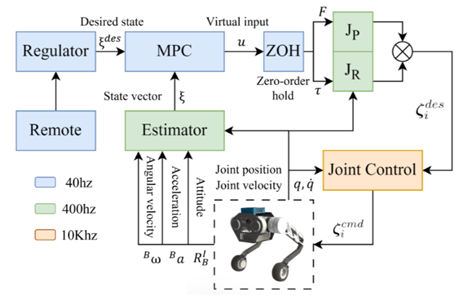
\includegraphics[width=0.7\textwidth]{figures/ch01/image18.png}
  \caption{HotWheel 控制框架}
\end{figure}

2025 年，Hao Xia 在跳跃控制方面提出了一套集成了轨迹规划与空中姿态控制的综合解决方案\cite{xia2025jump}。首先，它通过轨迹规划实现了对特定跳跃高度的精确控制，并设计了基于阻抗控制的轨迹跟踪器与跳跃状态观测器，确保了起跳与着陆阶段的稳定性。特别地，研究首次为双轮足机器人建立了一个专门的空中动力学模型，并基于此设计了空中姿态控制器，有效抑制了因腿部伸缩引起的机体俯仰与摆动，显著提升了跳跃过程的稳定性与可靠性，并通过实物实验验证了其优越性能。

\begin{figure}[H]
  \centering
  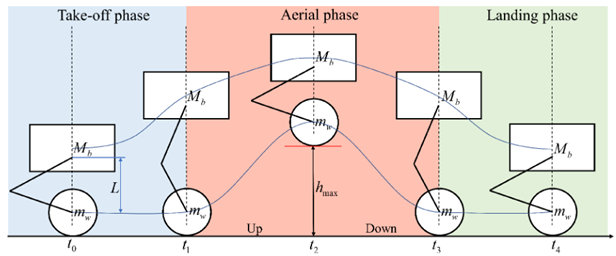
\includegraphics[width=0.72\textwidth]{figures/ch01/image19.png}
  \caption{跳跃过程及轨迹规划示意图}
\end{figure}

尽管 WBC、MPC 和 RL 等高级控制方法在性能上各具优势，但它们普遍存在对高精度模型（WBC、MPC）或海量训练数据（RL）的重度依赖，以及伴随而来的高计算复杂度问题，这在一定程度上限制了其在计算资源受限或模型不确定性高的场景下的应用。一种更具前景的控制思路，是转向轻量级、基于物理直觉的混合控制方案。
